\section{Technologie zastosowane w~pracy}

W~itym podrodziale wymienione zostały technologie zastosowane podczas tworzenia serwisu aukcyjnego będącego celem pracy.

\subsection{Ruby oraz Ruby~on~Rails} \label{technologie.baza}

\subsubsection{Ruby 1.9.3} \label{technologie.ruby}

\textit{Ruby} (ang.~rubin) to interpretowany, w~pełni obiektowy i~dynamicznie typowany język programowania stworzony w~1995 roku przez Yukihiro Matsumoto (pseudonim Matz). Wersja 1.9.3 cechuje się szybszym interpreterem, mniejszą konsumpcją zasobów oraz~drobnymi poprawkami w~standardowych bibliotekach języka.

\subsubsection{Ruby~on~Rails 3.1.0} \label{technologie.ror}

\textit{Ruby~on~Rails}\cite{ror} (często nazywany \textit{RoR} lub po~prostu \textit{Rails}) to~framework \textit{open~source} służący do~szybkiego tworzenia aplikacji webowych stworzony głównie przez duńskiego programistę Davida Heinemeiera Hanssona w~ramach pracy nad oprogramowaniem \textit{Basecamp}\cite{basecamp}. \textit{Rails} to~w~pełni wyposażone środowisko do~tworzenia aplikacji internetowych opartych o~bazy danych zgodnie ze~wzorcem \textit{MVC} (ang.~Model-View-Controller). \textit{Ruby~on~Rails} daje programiście środowisko w~pełni oparte o~język programowania \textit{Ruby} -- od~\textit{Ajax} dostępnego w~widokach (ang.~View), do~zapytania i~odpowiedzi w~kontrolerach i~logice biznesowej modeli.


Tuż po~pojawieniu się \textit{Ruby~on~Rails} na~forum publicznym okrzyknięto go~sensacyjnym. Tim O'Reilly, Założyciel O'Reilly Media mówił\cite{cytaty} ,,Ruby on Rails jest przełomem w~dziedzinie programowania aplikacji internetowych. Potężne aplikacje, których tworzenie do~tej pory zabierało tygodnie czy miesiące, są~teraz tworzone dosłownie w~kilka dni.''


Niestety -- w~ciągu ostatnich trzech lat spadło zainteresowanie technologią \textit{Ruby~on~Rails} (rys.~\ref{fig.wykres.googleresearch}). Programiści coraz rzadziej sięgają po~ten produkt wybierając nowsze rozwiązania takie jak \textit{Django}\cite{django} napisane w~języku \textit{Python}\cite{python}. Nadzieją na~poprawienie tej sytuacji jest nowo wydana -- trzecia wersja frameworku \textit{Ruby~on~Rails} oraz~ciągły rozwój dodatków -- wtyczek \texttt{gem}.

\begin{figure}[!t]
\centering
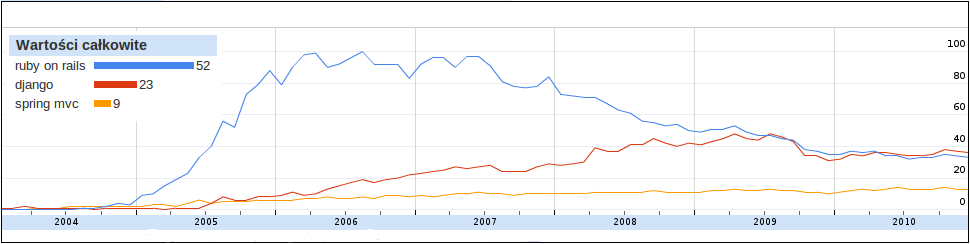
\includegraphics[width=\textwidth]{obrazki/googleresearch.png}
\caption[Statystyki Google na temat aplikacji szkieletowych]{Statystyka wyszukiwarki Google na~temat znanych aplikacji szkieletowych\cite{google.stats}}
\label{fig.wykres.googleresearch}
\end{figure}

\subsubsection{RSpec + Cucumber}

\textit{RSpec}\cite{rspec} to~narzędzie do~testownia oprogramowania pod względem testów jednostkowych oraz~behawioralnych przydatne w~realizowaniu projektów \textit{Test Driven Developement} oraz~\textit{Behavior Driven Developement}. Narzędzie \textit{Cucumber}\cite{cucumber} pozwala na~testowanie oprogramowania na podstawie tzw. scenariuszy -- dokumentów napisanych w języku naturalnym opisujących krok po~kroku funkcjonalności projektu.

% gemy, rozszerzenia, pluginy, dodatki, etc.

\subsection{Gemy i pluginy} \label{technologie.gemy}

\texttt{Gem} to~wtyczka (ang.~plugin), rozszerzenie dla aplikacji napisanych w jezyku \textit{Ruby}. \textit{Gemy} są~w~łatwy sposób zarządzane przez narzędzie \texttt{rubygems} pozwalające na pobieranie dowolnej wersji \textit{gemów} z~repozytoriów.


Do~realizacji celów pracy wykorzystano następujące wtyczki:

\begin{enumerate}
  \item \texttt{haml}\cite{haml} to plugin pozwalajacy na~użycie eleganckiego metajęzyka opisującego strukturę dokumentów HTML.
  \item \texttt{sass}\cite{sass} to podobny w działaniu do \texttt{haml} plugin obsługujący szablony CSS.
  \item \texttt{device}\cite{devise} to system obsługi autentyfikacji użytkowników (rejestracja, sesje, zarządzanie hasłami itp.) dla frameworku Ruby~on~Rails.
  \item \texttt{will\_paginate}\cite{will.paginate} to plugin obsługujący paginację stron.
  \item \texttt{tiny\_mce}\cite{tiny.mce} to plugin napisany w~języku JavaScript pozwalający na~użycie wewnętrznego edytora HTML na~stronach internerowych.
  \item \texttt{sqlite3}\cite{sqlite3} to relacyja baza danych z~możliwością użycia jezyka zapytań SQL; jest lekka i~szybka, czechuje się tym że bazy danych przechowywane są~w~osobnych plikach. Posiada swój własny adapter na~platformę Ryby~on~Rails.
\end{enumerate}

% technologie webowe

\subsection{Technologie W3 i poboczne} \label{technologie.web}

\textit{W3}\cite{w3} to~organizacja mająca na~celu opracowanie i~publikację dokumentacji standardów rządzących technologiami wykorzystywanymi do~tworzenia stron internetowych.

\begin{enumerate}
  \item \texttt{XHTML5}\cite{html5doc} (ang.~HyperText Markup Language version 5) jest językiem określającym strukturę stron internetowych. Składniowo bazuje on~na~języku XML (jest podzbiorem języka XML). Wersja piąta zapewnia kompatybilność wsteczną względem poprzednich wersji, a~przy tym precyzuje niejasności wersji 4 powodujące nieoczekiwane zachowanie wyświetlanych obiektów w~niektorych przeglądarkach.
  \item \texttt{CSS3}\cite{css3doc} (ang.~Cascade Style Sheet version 3). CSS3 jest językiem określającym wygląd elementów języka XML jaki wyświetlany jest w~przeglądarce. Wersja 3 zapewnia kilka dodatkowych opcji, jak np. \textit{grid layouts} (szablony pozycjonowane na bazie siatki)\footnote{\url{http://www.w3.org/TR/css3-grid/}}, \textit{shadows and rounded borders} (cienie obiektów, zaokrąglenia obramowania)\footnote{\url{http://www.w3.org/TR/css3-background/}}, itp.
  \item \texttt{JavaScript} jest lekkim, zorientowanym obiektowo wieloplatformowym językiem skryptowym. JavaScript, mimo że~nie jest użyteczny jako samodzielny język, został stworzony z~myślą o~łatwym zagnieżdżaniu w~innych produktach i~aplikacjach, jak na~przykład przeglądarki internetowe. JavaScript może zostać powiązany z~wewnętrzną strukturą danego środowiska dając programiście swobodną kontrolę nad jego elementami.
  \item \texttt{AJAX} (ang. Asynchronous JavaScript and XML) to technologia tworzenia aplikacji internetowych, w~której interakcja użytkownika z~serwerem odbywa się bez przeładowywania całego dokumentu, w~sposób asynchroniczny. Ma~to~umożliwiać bardziej dynamiczną interakcję z~użytkownikiem niż w~tradycyjnym modelu, w~którym każde żądanie nowych danych wiąże się z~przesłaniem całej strony HTML.
  \item \texttt{jQuery}\cite{jquery} (z.~ang. query -- zapytanie) -- lekka biblioteka programistyczna dla języka JavaScript, ułatwiająca korzystanie z~JavaScript (w~tym manipulację drzewem DOM). Kosztem niewielkiego spadku wydajności w~stosunku do~profesjonalnie napisanego kodu w~niewspomaganym JavaScripcie pozwala osiągnąć interesujące efekty animacji, dodać dynamiczne zmiany strony, wykonać zapytania AJAX. Większość pluginów i~skryptów opartych o~jQuery działa na~stronach nie wymagając zmian w~kodzie HTML (np.~zamienia klasyczne galerie złożone z~miniatur linkujących do~obrazków w~dynamiczną galerię). Wszystkie efekty osiągnięte z~pomocą jQuery można osiągnąć również bez jej użycia. Jednak kod okazuje się nieporównywalnie dłuższy i~bardziej skomplikowany.
\end{enumerate}
